%% Fiktivní kapitola s ukázkami sazby


\chapter{Návrh řešení}


V této kapitole je popsán návrh technického řešení uvedených problémů.


\section{Úvod}


Běh celé aplikace bude rozdělen do dvou částí.


\begin{itemize}
\item Stahování a ukládání real-time dat o polohách vozidel do databáze, které budou doplněny o odhad zpoždění pro okamžité zveřejnění v uživatelské aplikaci.


\item Modelování profilů jízd jednotlivých úseků. Tyto modely budou pak dále sloužit k odhadování zpoždění v budoucnu. Výpočet modelů bude prováděn jednou za delší časový úsek (nejlépe jednou za den).
\end{itemize}


Protože obě části jsou na sobě závislé v iniciálním běhu bude prováděna první část sběru dat bez odhadu zpoždění, nebo pomocí již existujícího triviálního lineárního odhadu.

\section{Architektura}


Schéma návrhu celé aplikace a komunikační mapa jednotlivých komponentů je ilustrována na diagramu \ref{fig:design_diagram}.


\begin{figure}
\centering
  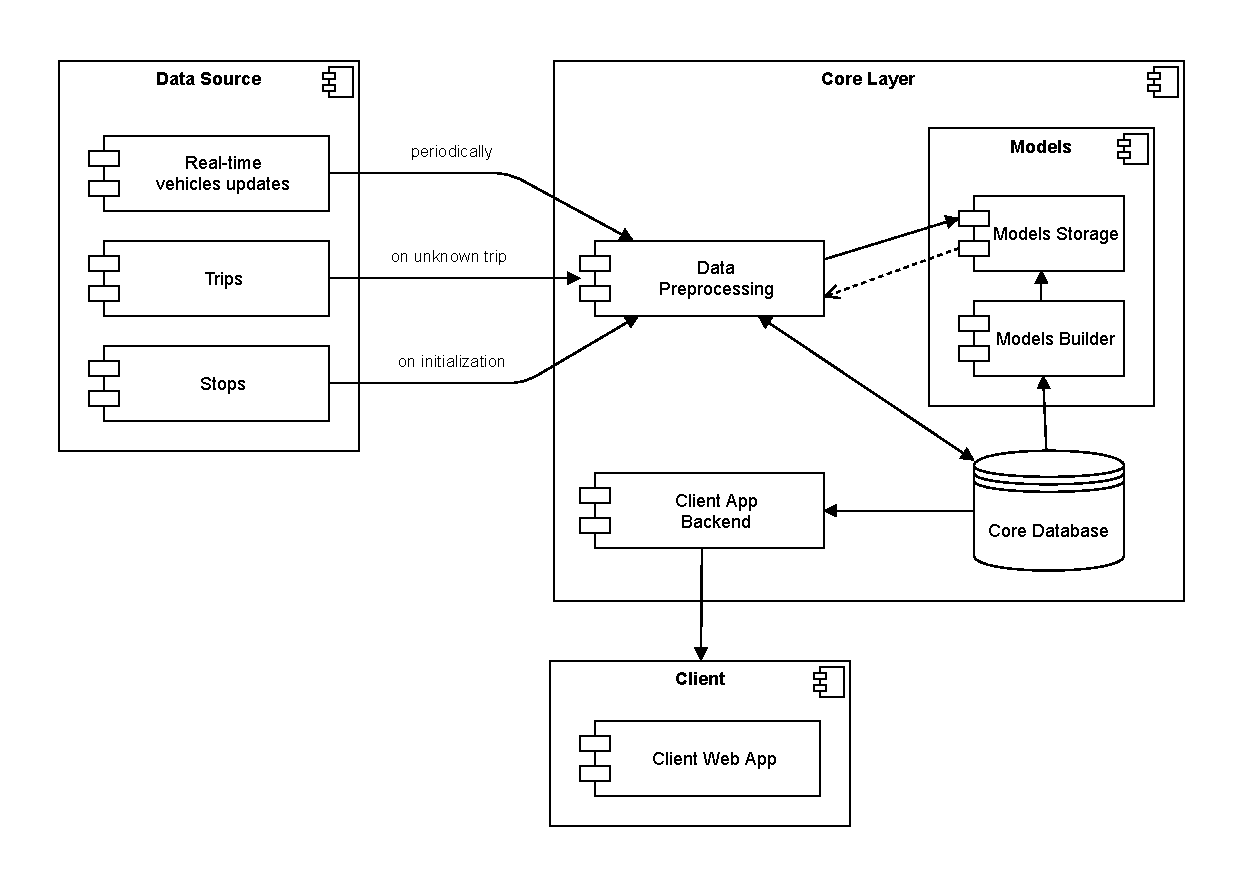
\includegraphics[width=\linewidth]{../img/design_diagram}
  \caption{UML diagram návrhu aplikace}
  \label{fig:design_diagram}
\end{figure}


\bigbreak


Návrh architektury vychází z popsaných funkčních požadavků a analýzy dat.


\bigbreak


Moduly Data Preprocessing a Client App Backend musí být odděleny, protože přistupují do databáze nezávisle. Z logiky věci: stahování dat databázi plní a back-end klientské aplikace data z databáze čte.


\bigbreak


Modul starající se o modely je také oddělen od zbytku systému, protože bude volán zcela nezávisle na stahování dat i back-endu klientské aplikace. Konstrukce modelů bude číst data z databáze a vytvořené modely ukládat na disk počítače. Program plnící databázi pak bude pouze číst tyto vytvořené modely a pomocí nich odhadovat zpoždění.

\bigbreak

Odhadnuté zpoždění se spočítá v modulu Data Preprocessing při zpracování každého jednotlivého spoje, poté se spolu s ostatními daty o spoji vloží do databáze jako aktuální zpoždění daného spoje.


\section{Zpracování vstupních dat} \label{section:zpracovani_vstupnich_dat}


Struktura uložení dat se bude zakládat na struktuře zdrojových dat popsaných v kapitole \ref{chapter:analyza_zdroje}.


\bigbreak


Na datové platformě jsou historická real-time data o vozidlech dostupná řádově v jednotkách minut, což je naprosto nedostatečné pro jakékoliv pozdější využití v rámci této práce. Především pro počítání statistik a modelování profilů jízd nad daty je potřeba zřídit lokální databázi, která bude držet historická data tak, jak byla obdržena ze zdroje. Navíc data jsou poskytována ve formátu \gls{json}, který svou povahou není zrovna úsporný, co se do velikosti souboru týče. Proto je vhodné zvolit ukládání dat v jiném formátu.


\subsection{Databáze} \label{subsection:databaze}

Za tímto účelem tato práce bude využívat relační databázi obsluhovanou dotazovacím jazykem \gls{sql}. Struktura databáze je navržena na \gls{er} diagramu \ref{obr:ER}. Tento návrh vychází ze struktury vstupních dat a požadavků na softwarové řešení. Tato databáze se skládá z 5 tabulek. Jsou jimi:


\begin{figure}[p]\centering
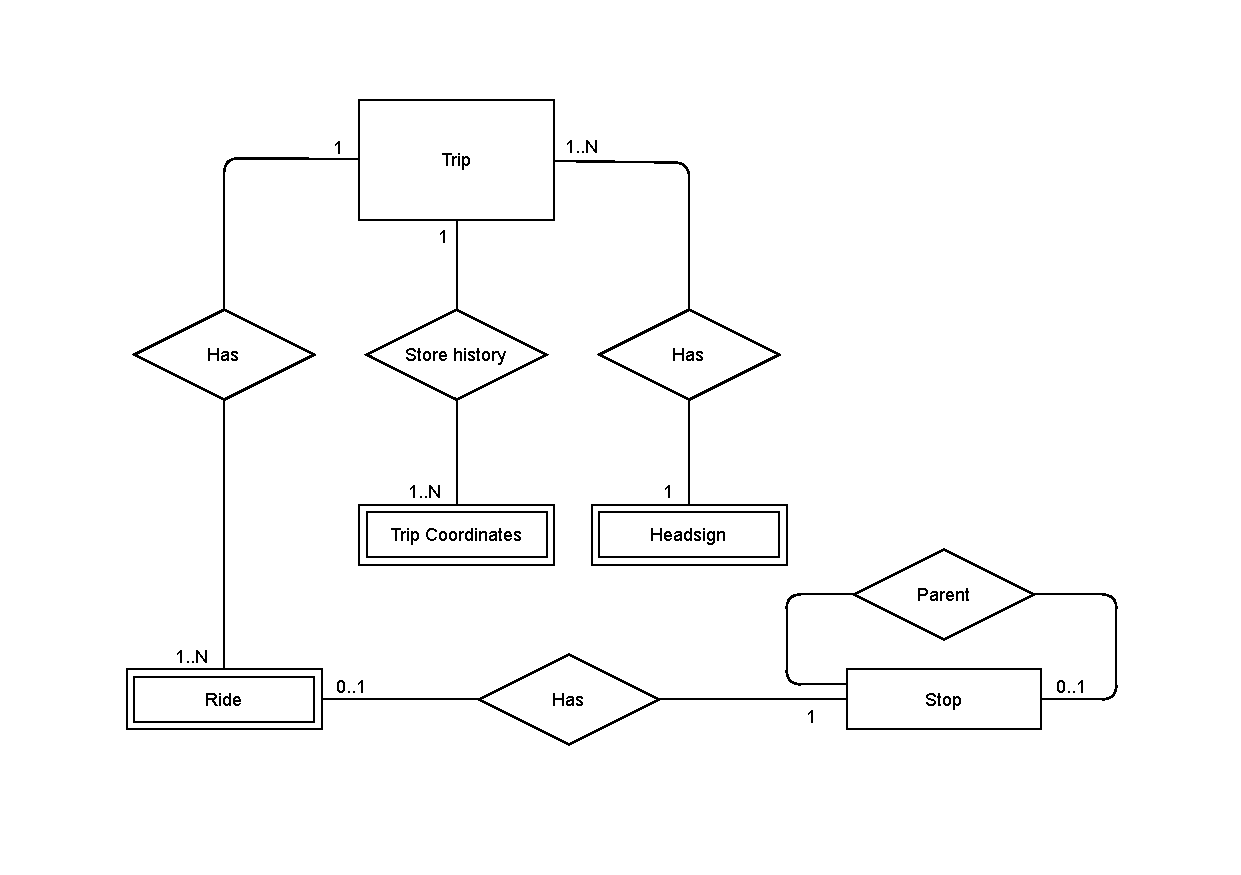
\includegraphics[width=\linewidth]{../img/er_diagram}
\caption{ER diagram návrhu databáze}
\label{obr:ER}
\end{figure}


\begin{itemize}
\item \verb-trips- všechny objevené jízdy


\begin{itemize}
\item \verb-id_trip- unikátní identifikátor používaný v databázi


\item \verb-trip_source_id- identifikátor tripu převzatý ze zdroje dat


\item \verb-id_headsign- identifikátor nápisu pro daný trip


\item \verb-current_delay- aktuální zpoždění tripu


\item \verb-shape_dist_traveled- aktuální vzdálenost ujetá od výchozí stanice


\item \verb-last_updated- čas poslední aktualizace, převzatý ze zdroje dat


\item \verb-trip_no- číslo dané linky
\end{itemize}


\item \verb-headsigns- nápisy nad vozidlem, cílová stanice


\begin{itemize}
\item \verb-id_headsign- unikátní identifikátor nápisu


\item \verb-headsign- text nápisu
\end{itemize}


\item \verb-trip_coordinates- všechna historická real-time data


\begin{itemize}
\item \verb-id_trip- identifikátor tripu, ke kterému se záznam váže


\item \verb-lat- zeměpisná šířka polohy vozidla


\item \verb-lon- zeměpisná délka polohy vozidla


\item \verb-inserted- čas vložení záznamu


\item \verb-delay- zpoždění zachycené v poslední projeté stanici před pořízením záznamu


\item \verb-shape_dist_traveled- vzdálenost ujetá od výchozí stanice tripu


\end{itemize}


\item \verb-stops- všechny zastávky


\begin{itemize}
\item \verb-id_stop- unikátní identifikátor zastávky


\item \verb-trip_source_id- identifikátor zastávky převzatý ze zdroje dat


\item \verb-parent_id_stop- identifikátor rodičovské zastávky, pokud existuje


\item \verb-stop_name- název zastávky


\item \verb-lat- zeměpisná šířka polohy zastávky


\item \verb-lon- zeměpisná délka polohy zastávky


\end{itemize}


\item \verb-rides- Je tabulka jízdního řádu každého spoje, tvořená seznamem zastávek s časy odjezdů a příjezdů. Pořadí zastávek, v jakém jsou spojem obslouženy, je určeno časem příjezdu, resp. odjezdu nebo atributem \verb-shape_dist_traveled-. \label{table:rides}


\begin{itemize}
\item \verb-id_trip- identifikátor spoje


\item \verb-id_stop- identifikátor zastávky


\item \verb-arrival_time- čas příjezdu tripu do zastávky


\item \verb-departure_time- čas odjezduu tripu ze zastávky


\item \verb-shape_dist_traveled- vzdálenost zastávky od výchozí zastávky tripu


\end{itemize}


\end{itemize}


Ve zdroji dat jsou atributy se jménem \verb-source_id- unikátní identifikátor entit, nicméně z dokumentace zdroje nevyplývá, jakého jsou datového typu. Také proto je tento identifikátor ukládán jako textový řetězec, ačkoli je tvořen pouze číslicemi a podtržítky, není nikde zaručeno, že jej lze jednoduše převést na číselný kód. Takže pro lepší výkon databáze je použito automaticky generované id typu \gls{int}.


\bigbreak


Každá tabulka má několik indexů, které zlepšují výkon databáze při vkládání a hledání dat. Přirozeně indexovány jsou primární klíče, což jsou ve všech tabulkách unikátní identifikátory typu \gls{int}. Dále indexujeme také unikátní identifikátory přebírané ze zdroje dat. A všechny atributy, podle kterých vyhledáváme v databázi, ať už dotazem přímo z kódu aplikace nebo některou z funkcí napsanou přímo v jazyce \gls{sql}. Takové indexy jsou:


\begin{itemize}


\item \verb-headsigns.headsign- unikátní index, textová hodnota nápisu


\item \verb-trips.id_headsign.- pro vyhledání všech spojů s danou konečnou stanicí


\item \verb-trips.trip_source_id- pro vyhledávání spoje podle zdrojového id


\item \verb-rides.shape_dist_traveled- pro setřídění jízdního řádu
\item \verb-inserted- čas vložení záznamu


\item \verb-trip_coordinates.shape_dist_traveled- pro vybrání vzorků poloh mezi dvojicí zastávek


\end{itemize}


\bigbreak


Databáze je nastavená tak, aby umožňovala získat všechny potřebné informace o vozidlech, hlavně přístup k historickým real-time datům, a to separovaně pro dvojici referenčních bodů. K tomu se zejména využívá atribut \verb-shape_dist_traveled-, který označuje vzdálenost na trase od výchozí zastávky a je součástí vstupních dat jízdních řádů i aktuálních poloh vozidel.

\bigbreak

Konečnou strukturu vytvořené databáze najdeme na \gls{eer} diagramu \ref{fig:EER}. \gls{sql} dotazy na sestavení celé databáze jsou definovány v příloženém souboru database.sql. Pro testovací, debuggovací a demonstrační účely jsou vytvořeny navíc i jiné databáze, které jsou strukturou totožné jako produkční databáze.

\begin{figure}[p]\centering
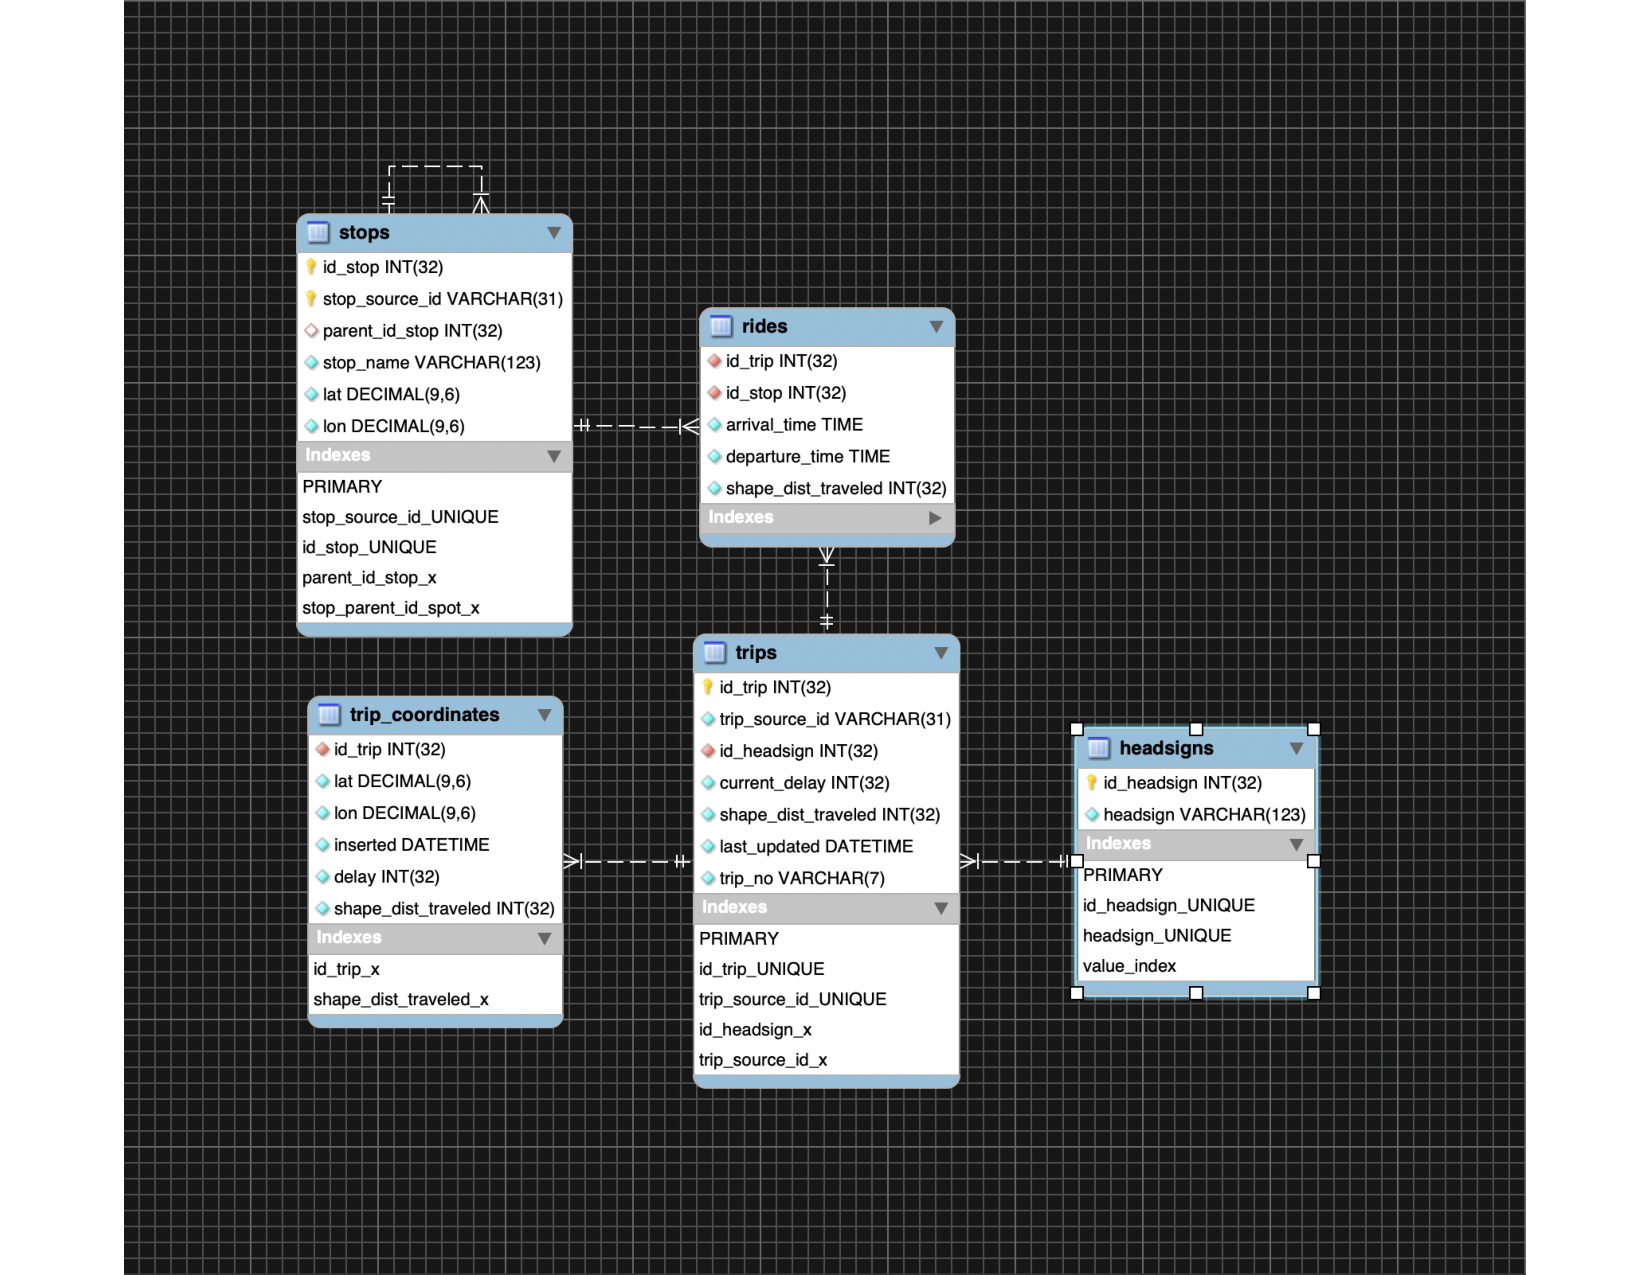
\includegraphics[width=\linewidth]{../img/eer_database}
\caption{ER diagram návrhu databáze}
\label{obr:EER}
\end{figure}

\subsection{Plnění databáze}


Tato databáze bude plněna skriptem, který bude naprogramován tak, aby vždy stáhl aktuální obraz dopravní situace a tato data uložil do databáze. Toto stahování z datové platformy probíhá podle následujícího algoritmu.


\bigbreak


Algoritmus:
\begin{code}[frame=none]
načti všechny dostupné zastávky
dokud skript běží
  načti aktuální polohy vozidel
  pro každé nalezené vozidlo
  pokud jízda vozidla je známá
    aktualizuj data o jízdě
  jinak
    stáhni informace o jízdě
    zpracuj a vlož jízdu do databáze
\end{code}


\bigbreak


Pokud se vyskytne jízda, která postrádá některou z požadovaných informací, je automaticky zahozena. Jelikož všechny informace ukládané do databáze, jsou důležité pro hlavní cíl této práce. Vkládání do databáze se provádí na několika místech v kódu aplikace, proto je toto řešeno pomocí databázových transakcí tak, aby stav databáze byl vždy konzistentní.


\bigbreak


Databázové transakce v obecném smyslu fungují tak, že můžeme měnit data v databázi (i více záznamů) a tyto změny se zapíší do samotné databáze až po potvrzení, že všechny změny byly provedeny správně. Pokud během provádění změn nastane chyba nebo zjistíme, že nám podstatné informace chybí, můžeme v jakékoli fázi provádění změn všechny dosud provedené změny zahodit a vrátit se do původního stavu databáze před započetím transakce.  Tedy pokud nejsou poskytnuta data ve formátu, který skript akceptuje, nebo nějaké povinné atributy chybí. Vložení celé jízdy nebude provedeno. Nejčastěji chybějící atribut je zpoždění v poslední zastávce.


\bigbreak


Mimo popsanou databázi se do určeného adresáře ukládají trasy jednotlivých jízd, která jsou ve formátu \gls{geojson} jako lomená čára definována souřadnicemi. Navíc data o trasách jsou používána pouze pro vizualizaci a jsou přijímána vizualizačním nástrojem ve formátu \gls{geojson}, tedy tyto data není nutné vůbec transformovat a není nutné je držet v hlavní databázi.


\section{Algoritmus odhadu zpoždění}


Z formulování problému vyplývá, že se má odhadovat zpoždění mezi dvěma referenčními body a jediné takové jsou zastávky na trase daného spoje. Cíl algoritmu může být tedy formulován, jako vytvoření popisu průběhu trasy mezi každou dvojicí zastávek, kterou alespoň jeden spoj obsluhuje a jsou bezprostředně sousedící ve sledu zastávek ve směru jízdy tohoto spoje. Nechť všechny dvojice zastávek a spoje je obsluhující splňující předcházející předpoklad označují jako $AB$ a $S$. Jedna dvojice zastávek pak bude $(a, b)$ a spoje je obsluhující se označují jako $S_{ab}$. První zastávku libovolné dvojce zastávek z $AB$ označíme $a$ a následující zastávku $b$.


\bigbreak


Z definice problému chceme modelovat jízdu vždy mezi danou dvojicí zastávek. Ke každé dvojici zastávek $(a, b)$ bude náležet jeden model, resp. modely pro pracovní dny a dny pracovního volna popisující průběh jízdy mezi nimi. Tyto modely budou vycházet z historických dat průjezdů mezi těmito zastávkami.


\bigbreak


Příklad takové dvojice zastávek $a$ a $b$ je uveden na příkladu v kapitole \ref{subsection:priklad_nelinearni_trasa}.


\subsection{Základní předpoklady} \label{section:zakladni_predpoklady}


Na začátku je potřeba ustanovit základní předpoklady, ze kterých bude vycházet sestrojený algoritmus vytvářející modely profilů jízd.


\bigbreak


Zastávky je potřeba rozlišovat na jednotlivá nástupiště. Toto výrazně nezvýší počet dvojic zastávek $AB$. Protože naprostá většina zastávek má pouze dvě nástupiště\footnote{Rozepsáno v kapitole \ref{subsubsection:zastavky}} -- pro každý směr jedno. Pokud má zastávka více nástupišť, je tak v případech, kdy ze zastávky odjíždí spoje do více směrů, a tudíž pro každé nástupiště je jiná následující zastávka -- počet dvojic $(a, b)$ se nezvýší. Z toho plyne zjednodušení, kterého se dopouštíme v průběhu celé práce, především pak pro tento algoritmus odhadu zpoždění a to tak, že termín zastávka a termín nástupiště splývají.


\bigbreak


Všechny spoje $S_{ab}$ bez ohledu na linku nebo dopravce jedou ze zastávky $a$ do zastávky $b$ po stejné trase a vzdálenost je tedy konstantní. -- Předpokládá se, že žádný dopravce nevyužívá jinou komunikaci a pro všechny platí pravidla silničního provozu stejně.


\bigbreak


Čas jízdy ze zastávky $a$ do $b$ závisí pouze na denní době a dne v týdnu. Navíc platí, že žádný z dopravců nedisponuje právem přednosti v jízdě před jiným dopravcem nebo výrazně výkonnějším vozidlem.  Dojezdové časy mohou být ovlivněny jen charakterem řidiče, avšak toto není zjistitelné z poskytnutých dat a zároveň se předpokládá, že charaktery řidičů jsou rovnoměrně rozloženy mezi všechny dopravce a linky. Podle jízdních řádů některé linky jedou ve stejnou denní dobu rychleji než jiné, avšak skutečná doba jízdy je stejná. Tím, že některý spoj zastávku pouze projíždí, a tedy je rychlejší než jiný spoj, není porušení tohoto předpokladu, protože se jedná o dvě různé dvojice zastávek.


\bigbreak


Během jízdy mohou nastat mimořádné události, které porušují výše uvedené předpoklady, nicméně detekce mimořádností a jejich řešení je nad rámec této práce a jejich počet je zanedbatelný. Proto na statistické modely nebudou mít vliv.


\subsection{Návrh modelování} \label{subsubsection:analyza_dat}


Na úvod uveďme, že ve všech grafech a následně i pro počítání modelů, byly všechny zobrazené vzorky poloh vozidel v grafech zarovnány tak, aby jejich jízda ze zastávky $a$ vždy začínala se zpožděním 0 sekund. To podle nahlášeného zpoždění v zastávce $a$.


\bigbreak


Z dat je však patrné, že ne vždy se zarovnání do nuly podařilo. Takové případy jsou pak způsobeny chybami v datech vysílaných z vozidel nebo špatně určeným zpožděním v poslední projeté stanici na straně poskytovatele dat. Takové chyby však vznikají spíše výjimečně, a proto ovlivňují statistické výpočty jen málo. Pro eliminaci těchto chyb je pak implementován modul, který se pokouší očividně chybné vzorky najít a smazat. To také z důvodu vizualizace vzorků v grafech, kde jeden vzorek, zcela mimo škálu jiných vzorků, rozhodí celý graf, který se tak stává nepřehledným.


\bigbreak


Dále si uvedeme druhy profilů jízd a způsoby jejich modelování.


\subsubsection{Lineární model}




Odhad zpoždění vozidla na trase se v současné době provádí pomocí lineárního modelu. Tedy s předpokladem, že vozidlo jede konstantní rychlostí po celou dobu jízdy mezi dvojicí zastávek $a$ a $b$.


\bigbreak


Ačkoli je snaha tento model nahradit lepším, v některých situacích může jeho použití i nadále dávat smysl. Zejména pak v případech, kdy není k dispozici dostatek dat, nebo je vzdálenost dvou zastávek natolik malá, že nemá smysl ani jakýkoliv odhad zpoždění dělat.


\subsubsection{Polynomiální profil jízdy}


Po analýze dat poloh vozidel a možných vlivů ovlivňující profil jízdy je patrné, že v průběhu jednoho dne dochází na trase nejvýše k několika výkyvům rychlosti jízdy. Viditelné jako "vlny" v průběhu dne na grafu \ref{fig:dojezd_ve_fazich_dne}), v 8:30 hod\footnote{časy jsou uvedeny v UTC}. Jízda trvala téměř 10 minut, naopak ve večerních hodinách jízda trvá kolem 7 minut.


\bigbreak


K tomuto dochází například v případech, kdy spoj zastavuje ve městě a v následujících několika málo kilometrech jede pomaleji, poté zrychlí a dále opět vjede do města. Takový model se hodí spíše na delší trasy s plynulou jízdou.


\begin{figure}
\centering
  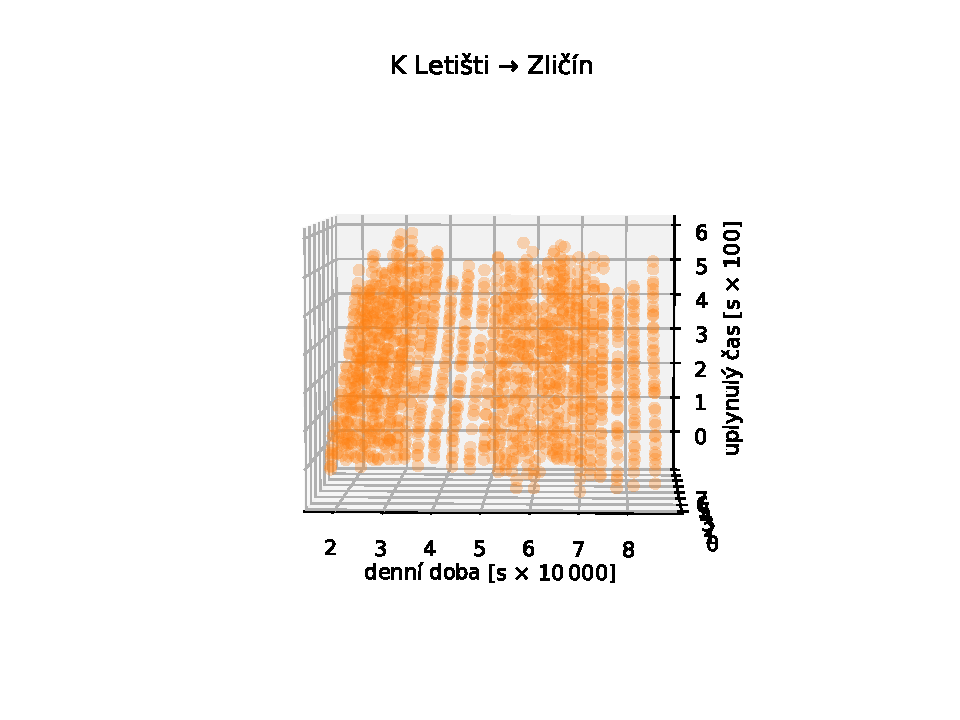
\includegraphics[width=\linewidth]{../img/dojezd_ve_fazich_dne}
  \caption{Variabilita délky jízdy v průběhu dne}
  \label{fig:dojezd_ve_fazich_dne}
\end{figure}


Stejně tak po analýze profilu jízdy v závislosti na ujeté vzdálenosti je na grafu \ref{fig:dojezd_podle_vzdalenosti} vidět, že čas jízdy narůstá také v jistých "vlnách".


\begin{figure}
\centering
  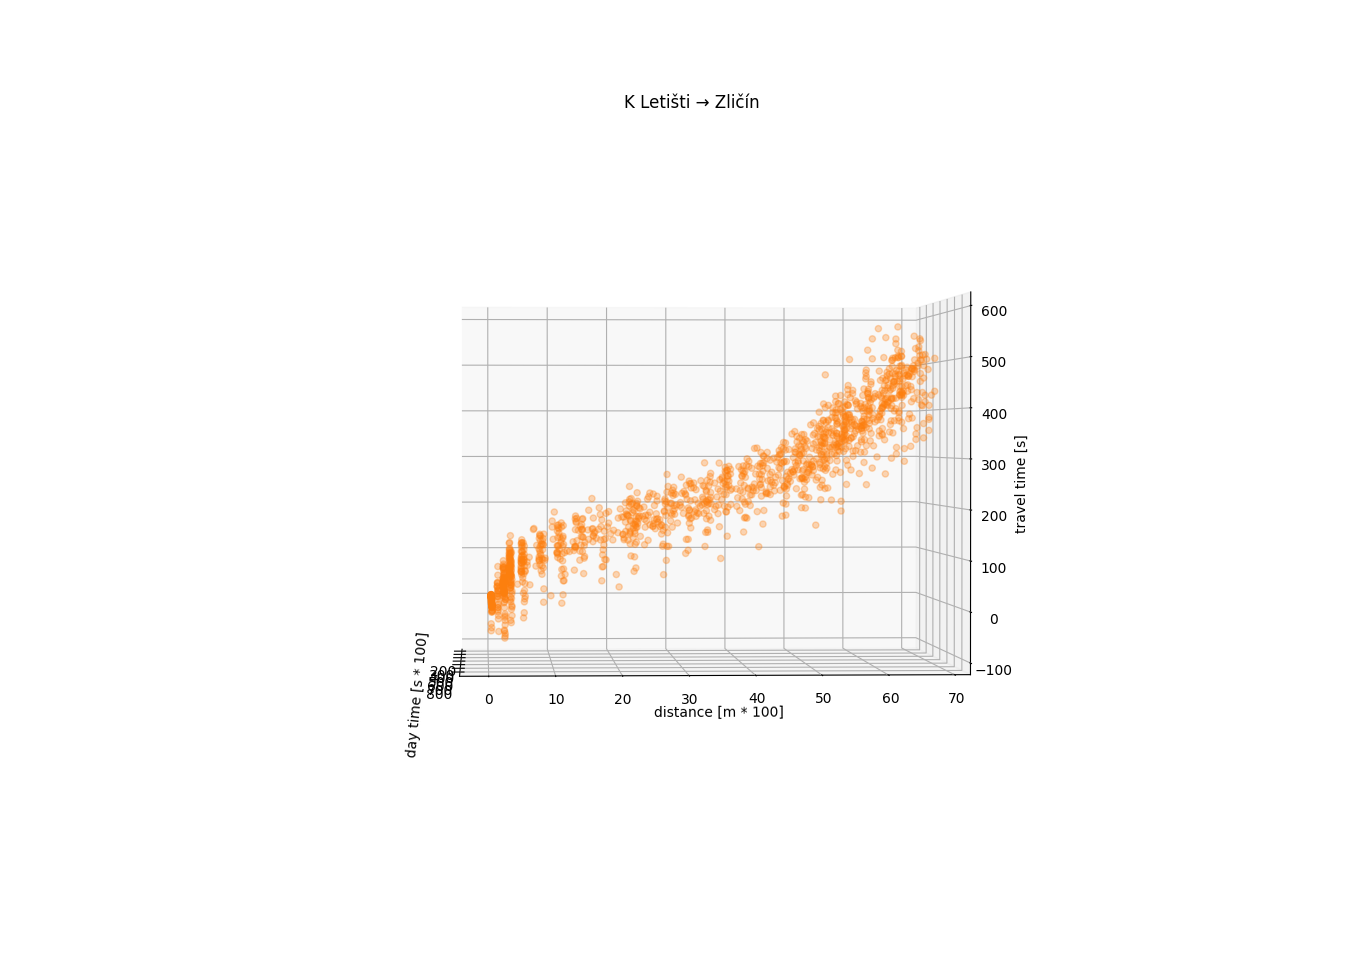
\includegraphics[width=\linewidth]{../img/dojezd_podle_vzdalenosti}
  \caption{Variabilita času jízdy v závislosti na ujeté vzdálenosti}
  \label{fig:dojezd_podle_vzdalenosti}
\end{figure}


Jak pozorujeme na grafech výše, je patrné, že vzorky poloh vytváří jisté vlny. Takové vlny se dají dobře popsat modely získané pomocí lineární regrese, resp. polynomiální regrese. Ve strojovém učení se k výpočtu polynomiální regrese využívá algoritmus lineární regrese s upravenými vstupními daty \citep[viz][Strany 265--268]{Gareth13}.


\bigbreak


Jako odhad zpoždění se pak vrací rozdíl skutečného počtu sekund na trase a predikce modelu. To celé se pak ještě přičítá k rozdílu predikce v modelu v čase a vzdálenosti příjezdu podle jízdního řádu a pravidelného příjezdu.


\bigbreak


Polynomiální model se tedy hodí pro situace, kdy je průběh trasy nějak ovlivněn vždy ve stejném úseku a má vliv na každý projíždějící spoj. Nebo se v průběhu dne pozvolna mění v závislosti na dopravním vytížení projížděných úseků.


Polynomiální model je pro představu vykreslen v grafu v úvodním příkladu v kapitole \ref{subsection:priklad_nelinearni_trasa}.


\subsubsection{Nepravidelné profily jízdy}


Výše popsaný příklad však ilustruje téměř ideální případ, kde je pravidelnost jízdy velmi dobře viditelná. Rozeberme si proto nyní i jiné druhy profilů jízd.


\bigbreak


Na grafu \ref{fig:cerny_most_chvaly} je patrné, že vzorky poloh vozidel profilu jízdy stále vytváří vlny. Ovšem už nejsou tak jednoznačně vidět jak v předchozím příkladě, a především se v celém grafu objevuje pár vzorků, které zcela vybočují mimo největší shluky vzorků. V těchto případech se zřejmě jedná o případy vozidel, které potkala nějaká anomálie při výjezdu ze stanice, a proto nabraly zpoždění hned na začátku.


\begin{figure}
\centering
  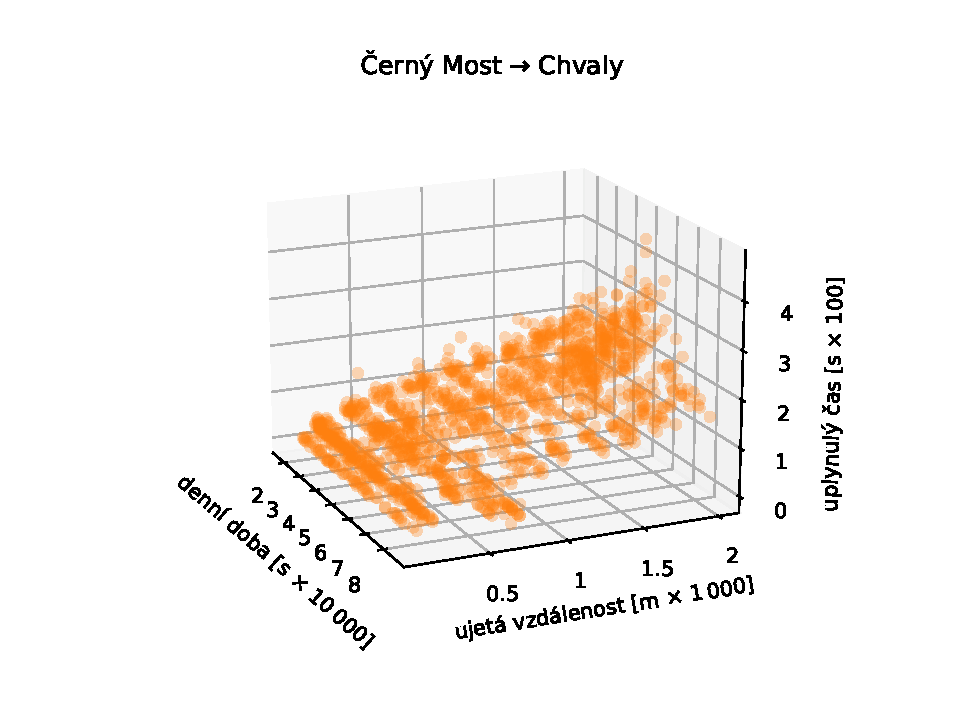
\includegraphics[width=\linewidth]{../img/4383_2712}
  \caption{Úsek s nepravidelnostmi}
  \label{fig:cerny_most_chvaly}
\end{figure}


Pro velmi krátké trasy se zobrazené vzorky dat mohou jevit jako zcela nepravidelné. Příklad uveden na grafu \ref{fig:divoka_sarka_veleslavin}. To je způsobeno tím, že doba jízdy trasy je natolik krátká, že jeden spoj trasu projede za minutu, ale druhý spoj, který se zdrží o zanedbatelný čas (z pohledu problému řešeného v této práci) přijede do následující stanice až za dvojnásobnou dobu. Dále je vysoký rozptyl vzorků způsoben nepřesnostmi při měření polohy vozidel a dalšími možnými problémy. Jelikož se ale jedná o velmi krátké trasy, nemá smysl jejich specifika vůbec řešit, protože spočítaná data by zastarala ještě před zveřejněním.


\begin{figure}
\centering
  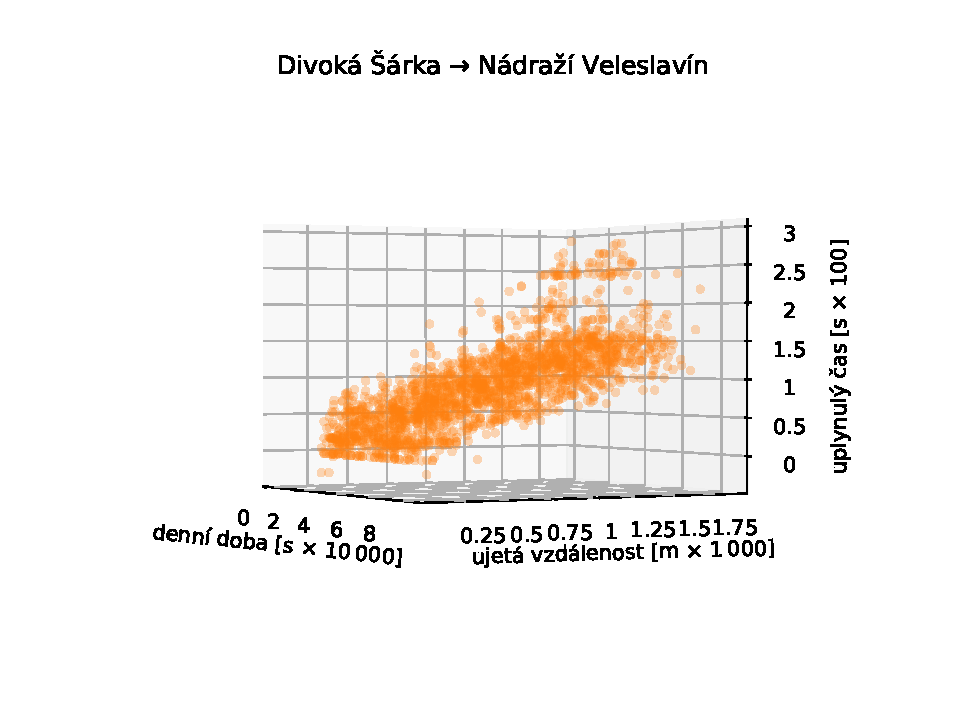
\includegraphics[width=\linewidth]{../img/164_165}
  \caption{Úsek s nepravidelnostmi 2}
  \label{fig:divoka_sarka_veleslavin}
\end{figure}

\bigbreak


Na ukázku uveďme ještě příklad grafu \ref{fig:delayed_trip}, kde jedna jízda dosáhla výrazného zpoždění oproti ostatním jízdám. Současně zde můžeme vidět poměrně častou chybu ve vstupních datech, kdy jedné jízdě přísluší vzorky poloh zcela mimo škálu grafu. Po bližším přezkoumání se jízda jeví, jakoby jela opačným směrem. V naší práci, ale nebudeme zkoumat zdroj chyby, ani se snažit data nějak opravit a rovnou tyto vzorky voloučíme.


\begin{figure}
\centering
  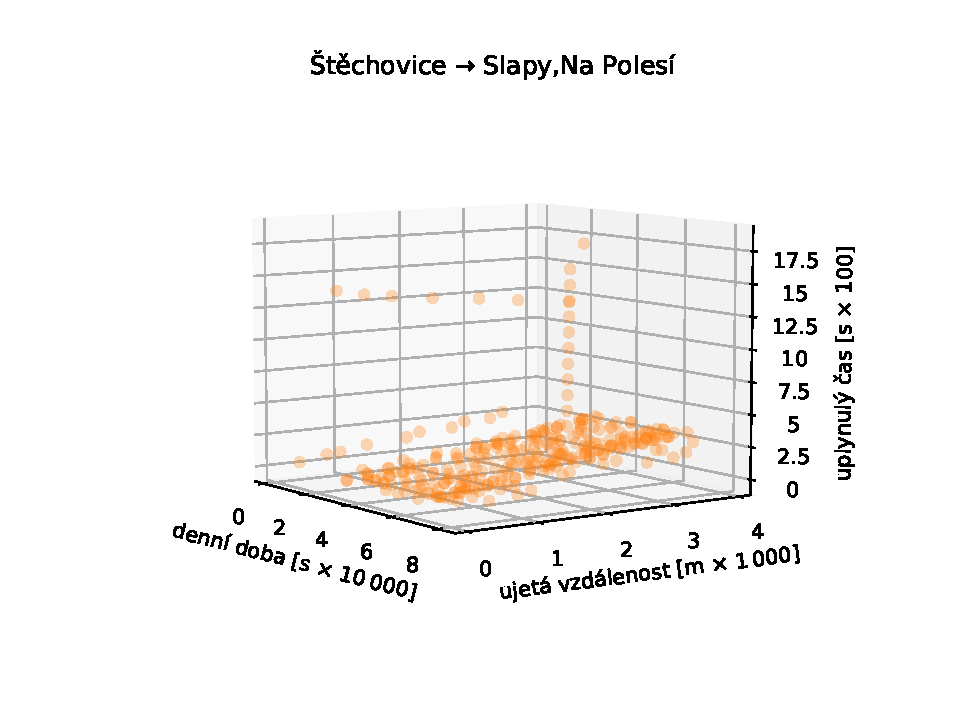
\includegraphics[width=\linewidth]{../img/16_17}
  \caption{Výrazné zpoždění jedné jízdy a chybný směr jízdy}
  \label{fig:delayed_trip}
\end{figure}


\subsubsection{Model konkávním obalem}


Na dalším grafu \ref{fig:nepredvidatelne_zdrzeni} je zobrazen příklad, kdy na trase existuje bod, který určité procento projíždějících spojů zdrží o netriviální dobu. Něco takového nastane, pokud spoje projíždí světelnou křižovatkou nebo místem kde se náhodně tvoří kolona vozidel. Zde dochází ke skokové změně průběhu bodové funkce. Spojité modely, jakým je polynomiální model, by s okolím tohoto kritického místa měly problém. Pro případy, kdy je na trase jen jeden takový bod by použití polynomiálních modelů vyhovovalo, byť by v bodě skoku odhad nebyl úplně přesný. Ale předpokládejme, že nalezená polynomiální funkce by tento skok zohlednila, ale teoreticky je potřeba algoritmus, který umí pracovat s více kritickými body na trase.


\begin{figure}
\centering
  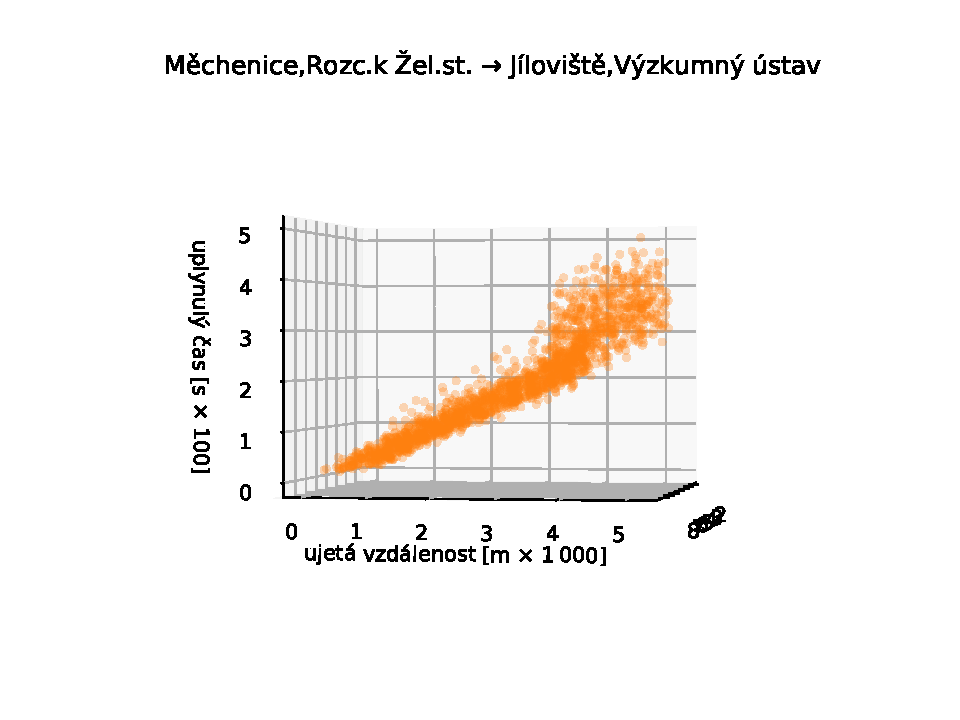
\includegraphics[width=\linewidth]{../img/1128_1129}
  \caption{Úsek s nepravidelným zpožděním}
  \label{fig:nepredvidatelne_zdrzeni}
\end{figure}


\bigbreak


Nevyhovující průběh trasy se dvěma kritickými body $x$ a $y$ na trase odpovídá následně popsané modelové situaci jízdy vozidel mezi dvěma zastávkami. Uvažme, že se většina projíždějících spojů zdrží pouze v prvním kritickém bodě $x$ o $c$ sekund, nebo pouze v druhém kritickém bodě $y$ o $c$ sekund, nebo se lehce zdrží v obou kritických bodech o $c_y + c_x = c$ sekund\footnote{$c_x$ značí nabrané zpoždění v bodě $x$, pro $y$ analogicky}. S takovým zdržením je počítáno v jízdním řádu a tedy vozidla, která projedou první kritický bod bez zdržení, jedou na čas stejně tak, jako vozidla v něm zdržená. O snížení nebo zvýšení případného zpoždění spoje je možno rozhodnout až po projetí druhého bodu. Zatímco polynomiální model by svými odhady jen uváděl uživatele v omyl.


\bigbreak

Ilustrujme výše popsané na modelovém příkladu na grafu \ref{fig:concave_hull}. Uvažujeme vozidlo jedoucí na trase mezi dvojicí zastávek, které jsou ve vzdálenosti 10 km. Pravidelný čas jízdy je 720 s. Na trase jsou 2 kritické body ve vzdálenosti 1.5 až 2 km a 8 až 8.5 km, ty si můžeme představit jako pomalu pojíždějící kolonu. Na tomto grafu máme vyobrazené 4 možné průjezdy této trasy: vozidlo projede bez zdržení, zdrží se pouze v bodě $x$, zdrží se pouze v bodě $y$ a zdrží se v obou bodech $x$ i $y$. O předjetí vozdila, které projede zcela bez zdržení, můžeme rozhodnout až po projetí bodu $y$. Stejně tak o zpoždění vozidla, které se zdrží v obou bodech, můžeme rozhodnout až v okamžiku zaseknutí se v bodě $y$. Všechny vzorky vozidel, které by se promítly do prostoru vyznačeného oranžovou barvou, mají z našeho pohledu nezměněné zpoždění.


\begin{figure}
\centering
  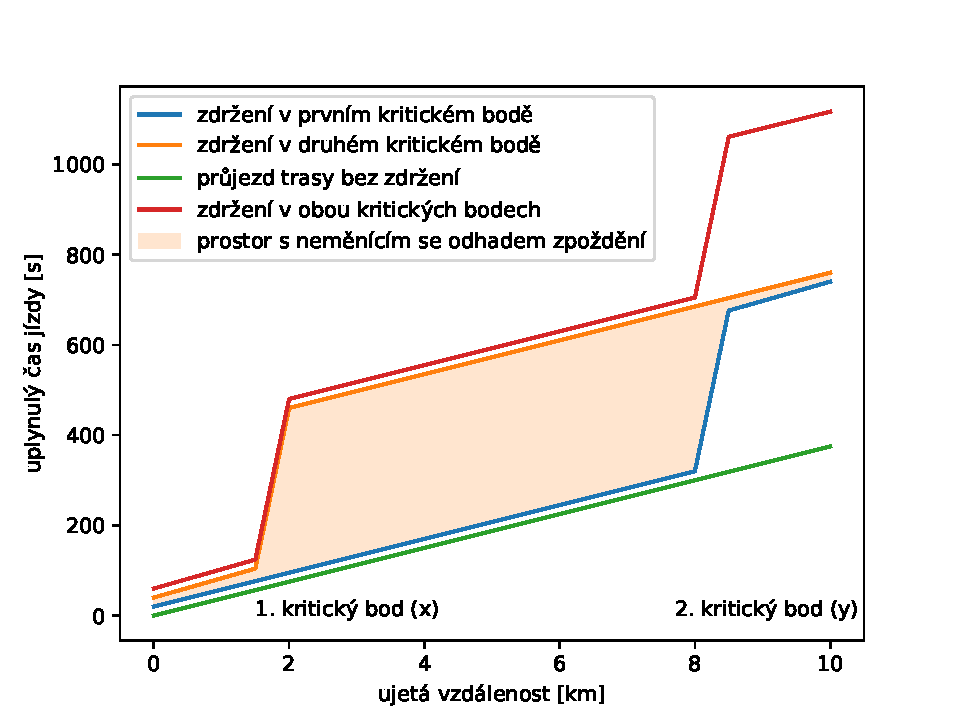
\includegraphics[width=\linewidth]{../img/concave_hull}
  \caption{Modelový příklad profilu trasy dobře popsatelného konkávním obalem}
  \label{fig:concave_hull}
\end{figure}


\bigbreak


Jinými slovy na grafu času jízdy a vzdálenosti od vyjetí ze zastávky vzniká jakýsi podprostor, v němž se zpoždění nemění. Pro ohraničení tohoto podprostoru je potřeba sestrojit konkávní obal všech vzorků u všech spojů, které přijely do následující zastávky včas.


\bigbreak


Nejprve k samotnému konkávnímu obalu je potřeba říct, že na množině bodů není definován jednoznačně, jak je vidět na obrázku \ref{fig:konkavni_obal_nejednoznacny} \citet{Asaeedi}. Pro účely této práce je zapotřebí, spočítat obal ve třídimenzionálním prostoru, což je velmi komplikovaný úkol a není ani snadné nalézt knihovny, které by konkávní obal ve 3D spočítaly. Proto je potřeba přijít se zjednodušením úlohy. Tedy počítat obal pouze pro dvoudimenzionální prostor. Toho se nedá dosáhnou jinak, než diskretizací úlohy a počítání obalu pro každou hodinu zvlášť, tedy ze všech bodů, které byly zaznamenány v průběhu jedné hodiny.


\begin{figure}
\centering
  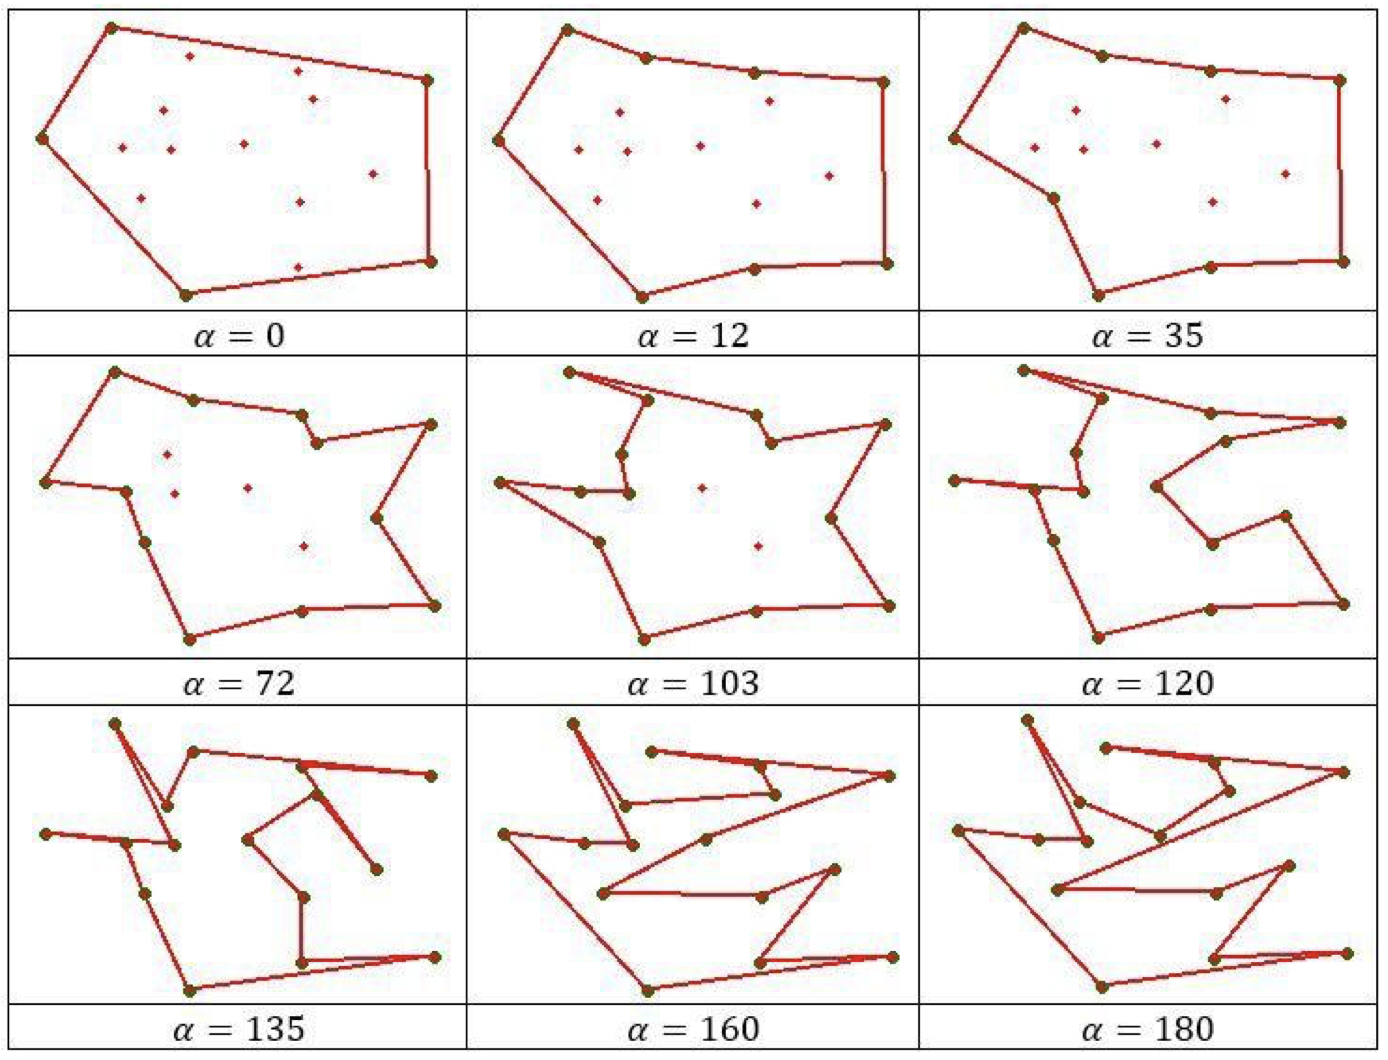
\includegraphics[width=0.8\linewidth]{../img/konkavni_obal_nejednoznacny.png}
  \caption{Nejednoznačnost konkávního obalu}
  \label{fig:konkavni_obal_nejednoznacny}
\end{figure}


\bigbreak


 Tím může dojít k vetší granularitě obalu, než by bylo vhodné, nicméně předpokládá se, že hodina je dostatečně dlouhý časový interval na to, aby zde byly zachyceny všechny druhy průběhu jízdy a zároveň je to dostatečně krátký interval na nezkreslování denních výkyvů v čase jízdy.


 \bigbreak


Dále se jako netriviální ukazuje detekce spojů, které přijely včas, a tedy všechny jejich body mají být předány k výpočtu obalu. Nabízí se použít data o všech spojích, které přijely do cílové zastávky s co nejmenším zpožděním, ale je nutné mít na paměti, že příjezdy podle jízdního řádu nemusí vůbec odpovídat realitě. Proto se zdá být nejlepším řešením použít data od spojů, které přijely ve stejnou dobu, jako je průměr všech příjezdů do cílové zastávky. Toho se docílí tak, že se poslední vzorky podle vzdálenosti všech spojů použijí pro odhad času příjezdu. Dále se pro každou hodinu použije určité procento nejbližších spojů k tomuto odhadu.


\bigbreak


Z předchozího popisu řešení ovšem vyplývá, že pro výpočet obalu jsou použity spoje, které ani zdaleka nemusely přijet včas jak, je požadováno. Ale předpokládá se, že se nepříliš vzdalují od průměrného času příjezdu. To, že střední zpoždění pro celý obal není nulové, se vyřeší sečtením odchylky průměrného příjezdu od příjezdu podle jízdního řádu a následně přičtení této konstanty k odhadnutému zpoždění. Každopádně to, že rozptyl příjezdů spojů zahrnutých ve výpočtu obalu může být netriviální, vyžaduje nahlížet na tento obal jako na lineární prostor pohybu zpoždění. Tedy, že odhad zpoždění pro bod nacházející se v obalu je lineárně závislý na vzdálenosti od hranice obalu, avšak protože je známo časové rozpětí příjezdu spojů použitých pro výpočet obalu, je možné tuto vzdálenost snadno přenést na skutečné zpoždění.


\bigbreak


Naštěstí pro nás se v průběhu analýzy dat o polohách spojů nepodařilo najít jediný případ dvojce zastávek, mezi kterými by došlo k popsané situaci -- výskytu dvou kritických bodů. Nebo tyto body jsou natolik nevýrazné, že by popsané řešení pomocí konkávního obalu nepřineslo žádné zlepšení odhadu zpoždění, ba naopak vzhledem k implementační náročnosti a množstvím chyb vznikajících při tak algoritmicky náročných úkolech by přesnost odhadu zpoždění zhoršilo. Možných vysvětlení, proč tato situace nenastává, se nabízí více. Zejména vlivem složitosti dopravní sítě a závislostí v ní je možné, že pokud se vozidlo zdrží v jedné koloně vozidel a na jeho trase je ještě jeden kritický bod, pak je velmi pravděpodobné, že se zdrží i v něm, protože hustota dopravy je ve stejném čase stejná na celé trase vozidla. Tedy mohou nastat dvě situace: 1. vozidlo projede oba kritické body bez zdržení v časech s mírnou úrovní dopravy, 2. vozidlo se zdrží v obou kritických bodech stejně v časech s vysokou úrovní dopravy. Tyto situace jsou pokryty v popisu profilu jízdy polynomiálním modelem. Další vysvětlení je, že popisované segmenty trasy (mezi zastávkami) jsou příliš krátké na to, aby se zde vyskytly 2 kritické body. Jiné vysvětlení může být, že se použije jistý druh práva přednosti v jízdě pro spoje \gls{vhd}, čímž se myslí ovládání světelných křižovatek ve prospěch těchto vozidel, čímž se eliminuje dopad na zpoždění průjezdu křižovatkou.


\bigbreak


Případ, kdy by model podle konkávního obalu přinesl zlepšení, je na grafu \ref{fig:good_to_concave_hull}, který zobrazuje spočítaný model pomocí polynomiální regrese. Polynomiální regrese se sice se skokovou změnou nevypořádala, jak jsme předpokládali. Ale jediný problém nastane na trase před kritickým bodem, kdy model bude všem vozidlům přisuzovat vyšší předjetí. Jak je ale vidět z grafu, odhad se oproti středu vzorků odchyluje nanejvýš o desítky sekund.


\begin{figure}
\centering
  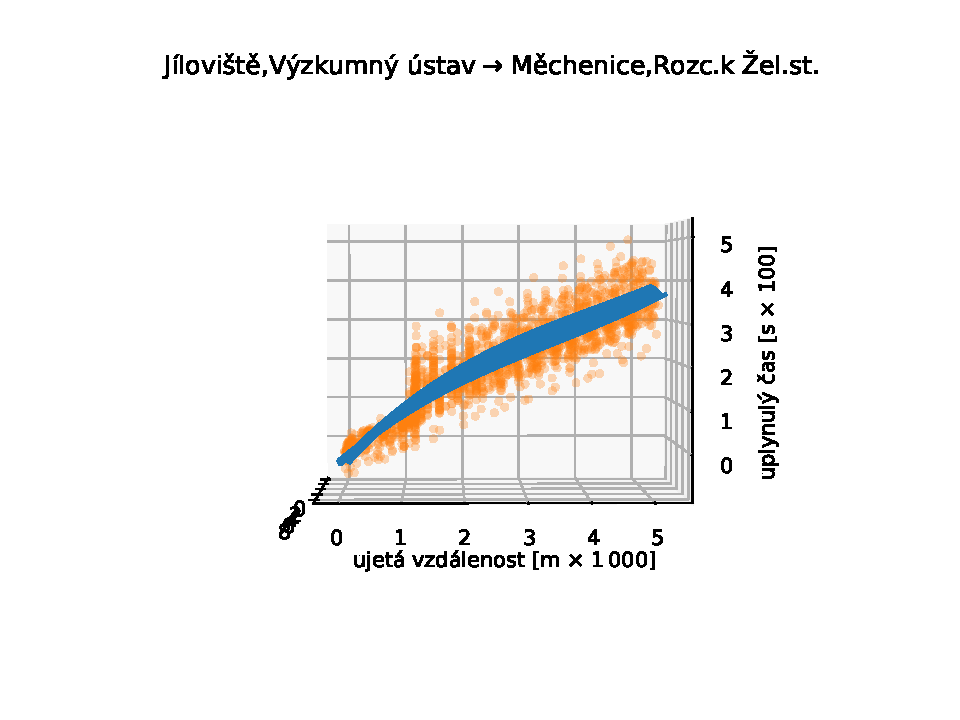
\includegraphics[width=\linewidth]{../img/8_9}
  \caption{Chyba polynomálního modelu}
  \label{fig:good_to_concave_hull}
\end{figure}


\bigbreak


Návrh algoritmu pracujícím s konkávním obalem je následující. Nejprve ukažme konstrukci konkávního obalu pro dvojici zastávek $a$ a $b$:


\begin{code}[frame=none]
poslední_vzorky = vyber všechny vzorky poloh vozidel
  těsně před dojezdem do stanice $b$ od všech spojů;
odhad_příjezdu = odhadni čas příjezdu v průběhu celého
  dne podle bodů v poslední_vzorky, např.: pomocí poly regrese;
spoje_včas = prázdné pole spojů;


pro každou hodinu h:
  spoje_včas += vyber spoje, které přijely nejblíže
    odhadu v hodině h;


konkávní_obal = prázdné pole


pro každou hodinu h:
  vzorky_poloh = vyber všechny body zaznamenané
    v hodině h a náležící kterémukoli spoji v spoje_včas;
  konkávní obal += spočítej konkávní obal z vzorky_poloh;


Vrací: konkávní_obal;
\end{code}


Dále odhad zpoždění z konkávního obalu. Pro funkci \verb-vzdálenost bodu od hranice obalu- se vždy myslí vzdálenost po kolmici na osu ujeté vzdálenosti a osu času dne.


\begin{code}[frame=none]
Vstup: bod v prostoru vzdálenosti, průběhu dne
  a času na trase (vzorek polohy vozidla)


pokud je bod v konkávní_obal:
  velikost_okna_příjezdu = rozdíl horní hranice obalu od spodní
    v zastávce příjezdu;
  spodek_okna = spodní hranice okna v čase
    příjezdu do zastávky;
  poměr = vzdálenost bodu od spodní hranice obalu
ku vzdálenosti bodu od horní hranice obalu;
  odhad_příjezdu = velikost_okna * poměr + spodek_okna;
jinak:
  pokud je bod pod obalem:
    odhad_příjezdu = spodek_okna - vzdálenost bodu od obalu;
  jinak:
    vrch_okna = horní hranice obalu
  v čase příjezdu do zastávky;
    odhad_příjezdu = vrch_okna + vzdálenost bodu od obalu;


Vrací: odhad_příjezdu - pravidelný příjezd;
\end{code}


\subsection{Využití modelů}


Z popsaných modelů v naší aplikaci budeme používat lineární model a polynomiální model. Rozhodnutí, který model využít, uděláme podle následujících faktorů.


\bigbreak


Pro všechny dvojice zastávek, které jsou blízko sebe, se použije lineární model, protože pro takovou vzdálenost nemá smysl počítat komplikovaný odhad a ani se zabývat možným způsobem odhadu. První důvod je, že takto krátké vzdálenosti mezi zastávkami jsou častým jevem ve městech, ale tento případ nechceme řešit ze stejných důvodů. Dále na těchto krátkých trasách, které mají i krátký čas jízdy velmi vynikají nepřesnosti v měření. Např. odchylka v měření 10 sekund na trase, jejíž projetí trvá 100 sekund, se projeví velmi výrazně.


\bigbreak


Lineární model zvolíme také v případě, že nemáme dostatek dat pro výpočet polynomiální modelu. Kolik dat je dostatečných se počítá jako funkce délky trasy a délka části dne ve které jsou zastávky obsluhované.


\bigbreak


Na závěr, pokud i přes počítání polynomiálního modelu zjistíme, že takový model má horší výsledky než model lineární, nemá smysl využívat polynomiální model.


\section{Vizualizace dat} \label{section:navrh_vizualizace}


 Aplikace vizualizace dat bude postavena z částí server a klient. Tedy serverová strana se postará o přístup k otevřeným datům z databáze na základě požadavků klienta.


\subsection{Návrh grafiky a UI}


Z výše popsaných funkčních požadavků budou vycházet grafické návrh uživatelského rozhraní. Předem je potřeba zdůraznit, že návrh do velkého detailu grafických a estetických vlastností této aplikace není předmětem této práce.


\bigbreak


Externí mapové podklady mohou být zobrazeny v několika barevných variacích, umožňují zobrazení ortofoto a také zobrazení s důrazem na různé mapové vrstvy. Pro nás je nejvíce žádoucí zobrazit vrstvu ulic a cest a dále pak určité orientační body jako jsou budovy, vodní plochy, lesy atp. Z palety barev je pak dobrou volbou neutrální béžová barva. Příklad takové mapy je na obrázku \ref{fig:mapbox_mapa}.


\begin{figure}
\centering
  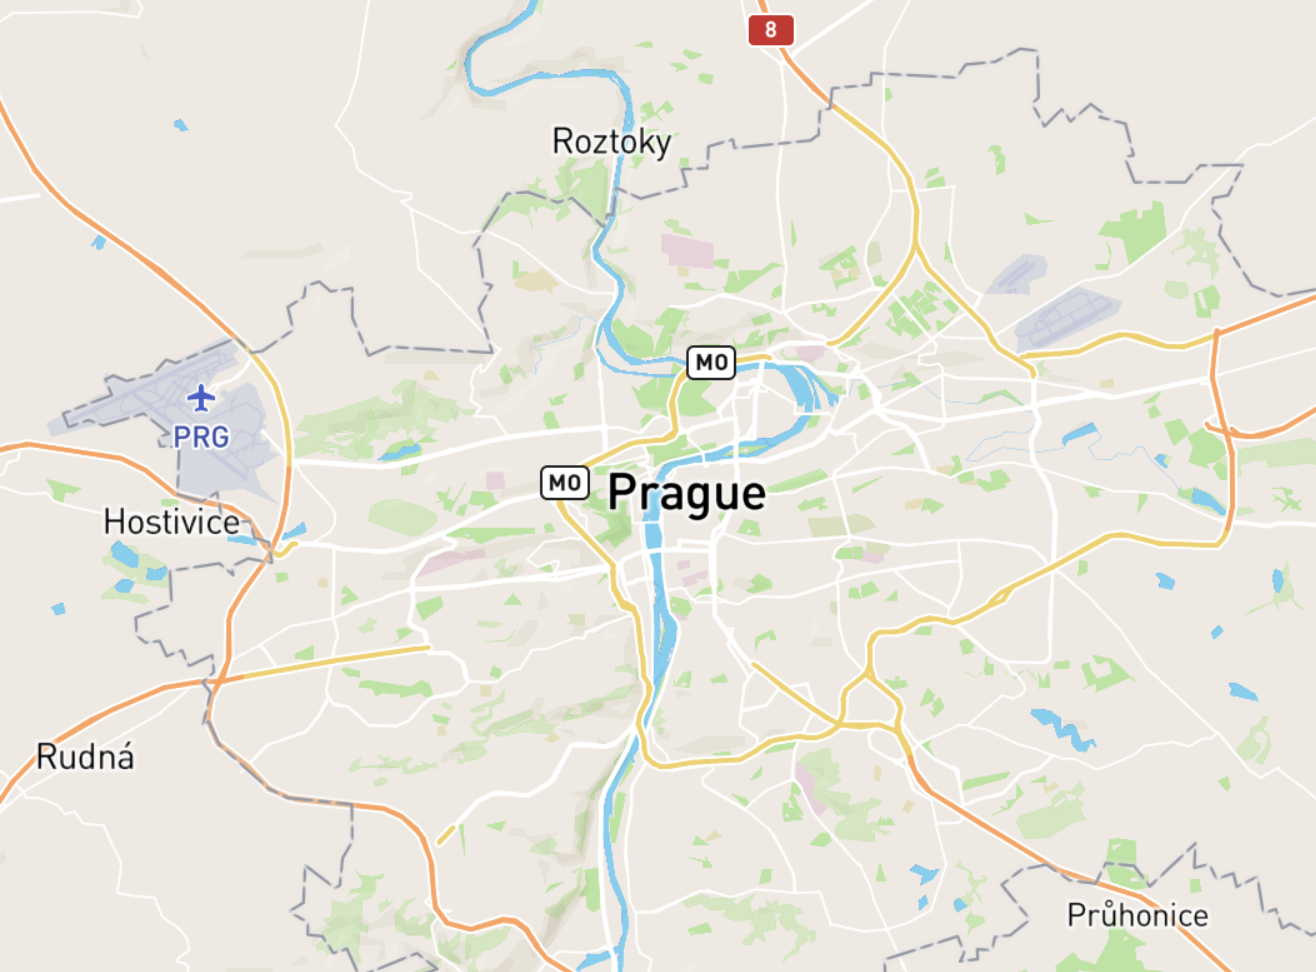
\includegraphics[width=0.5\linewidth]{../img/mapa_mapbox.png}
  \caption{Mapbox Mapa, použitý styl mapy: streets-v11}
  \label{fig:mapbox_mapa}
\end{figure}


Zobrazení jednotlivých spojů bude pomocí bodů v mapě, a to konkrétně barevným kruhem s číslem linky. Vybrané vozidla se rozliší jinou barvou a velikostí kruhu. Návrh reprezentace vozidel v mapě je zobrazen na obrázku \ref{fig:dve_vozidla}.


\bigbreak


Pro zvolené vozidlo se vykreslí celá jeho trasa včetně všech zastávek. Trasa je reprezentována lomenou čarou a zastávky jako špendlíky v mapě, po přejetí symbolu zastávky se zobrazí i její název. Za zvoleným vozidlem je zobrazena i historie jeho jízdy za uplynulých několik minut, to pomocí barevné lomené čáry, tvořící ocas zvoleného vozidla. Rovněž k povšimnutí na obrázku \ref{fig:dve_vozidla}.


\begin{figure}
\centering
  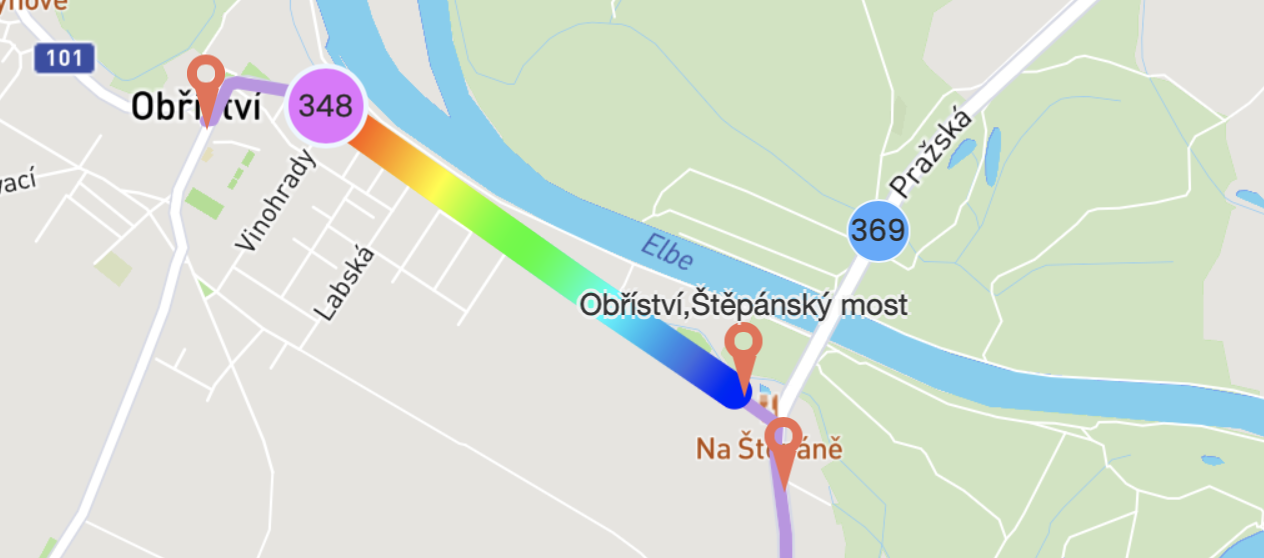
\includegraphics[width=0.5\linewidth]{../img/dve_vozidla.png}
  \caption{Design zobrazení elementů v mapě, linka je 348 je vybrána}
  \label{fig:dve_vozidla}
\end{figure}


Další informace o spoji, nebo zastávce se zobrazí v tabulce, která z části překryje mapu. Tato tabulka bude obsahovat informace o zvoleném vozidle, konkrétní konečnou stanici, jeho zpoždění a celý jízdní řád. Respektive informace o zvolené zastávce – název zastávky a všechny spoje, které zvolenou zastávkou budou projíždět včetně jejich pravidelného odjezdu a aktuálního zpoždění. Po kliknutí na zastávku\footnote{V tomto případě myslíme opravdu celou zastávku se všemi jejími nástupišti a nikoli pouze příslušné nástupiště. Protože se nemůžeme spolehnout na vytvořené relace označující všechny rodičovské nástupiště ve zdrojových datech, budeme za nástupiště příslušné jedné zastávce považovat nástupiště se stejným názvem.} se tedy zobrazí její odjezdová tabule.
